\documentclass{beamer}

%\setbeamersize{text margin left=7.5mm,text margin right=7.5mm}
\usepackage{tikz}

\usepackage{graphicx}
\usepackage[utf8]{inputenc}
\usepackage[T1]{fontenc}
\usepackage[english]{babel}
\usepackage{listings}
\usepackage{xcolor}
\usepackage{eso-pic}
\usepackage{mathrsfs}
\usepackage{url}
\usepackage{amssymb}
\usepackage{amsmath}
\usepackage{multirow}
\usepackage{subcaption}
\usepackage{hyperref}
\usepackage{booktabs}
\usepackage{eurosym}
\usepackage{bm}
\usepackage{cooltooltips}
\usepackage{colordef}
\usepackage{beamerdefs}
\usepackage{lvblisting}

\usepackage{algorithm}% http://ctan.org/pkg/algorithm
\usepackage{algpseudocode}% http://ctan.org/pkg/algorithmicx


% Shortcuts/Definitions
\DeclareMathOperator*{\argmin}{argmin}   % Jan Hlavacek
\DeclareMathOperator*{\argmax}{argmax}   % Jan Hlavacek
\newcommand{\matr}[1]{\mathbf{#1}} % undergraduate algebra version
%\newcommand{\matr}[1]{#1}          % pure math version
%\newcommand{\matr}[1]{\bm{#1}}     % ISO complying version


% Bibliography
\usepackage[backend=biber,sorting=nyt,style=authoryear]{biblatex}
\usepackage[autostyle,autopunct]{csquotes} % For Quotations
\renewcommand{\mkcitation}[1]{#1} % For correct footcites with csquotes
\addbibresource{references.bib}

\pgfdeclareimage[height=2cm]{logobig}{template/hulogo}
\pgfdeclareimage[height=0.7cm]{logosmall}{images/hulogo.pdf}


\setbeamercolor{block body alerted}{bg=alerted text.fg!10}
\setbeamercolor{block title alerted}{bg=alerted text.fg!20}
\setbeamercolor{block body}{bg=structure!10}
\setbeamercolor{block title}{bg=structure!20}
\setbeamercolor{block body example}{bg=green!10}
\setbeamercolor{block title example}{bg=green!20}
\setbeamertemplate{blocks}[rounded][shadow]

\renewcommand{\leftcol}{0.6}

\newcommand\myheading[1]{%
  \par\smallskip
  {\large\bfseries#1}\par\smallskip}




% Define Titlepage
\title[Elastic Full Procrustes Means for Sparse and Irregular Planar Curves]{Elastic Full Procrustes Means for Sparse and Irregular Planar Curves}

\authora{Manuel Pfeuffer}
\authorb{}
\authorc{}

\def\linka{}
\def\linkb{}
\def\linkc{}

\institute{Masters Thesis Presentation\\
Chair of Statistics\\
Humboldt--Universität zu Berlin}

\hypersetup{pdfpagemode=FullScreen}

\begin{document}

% 0-1
%%%%%%%%%%%%%%%%%%%%%%%%%%%%%%%%%%%%%%%%
\frame[plain]{
\titlepage
Advisors: Lisa Steyer, Almond Stöcker, Prof.\ Dr.\ Sonja Greven\\
\vspace{0.5em}
2nd Examiner: Prof.\ Dr.\ Nadja Klein
}


% 0-2
%%%%%%%%%%%%%%%%%%%%%%%%%%%%%%%%%%%%%%%%
\frame{
\frametitle{Motivation}
Calculate \alert{shape means} for \alert{2D curves}:
\begin{figure}
  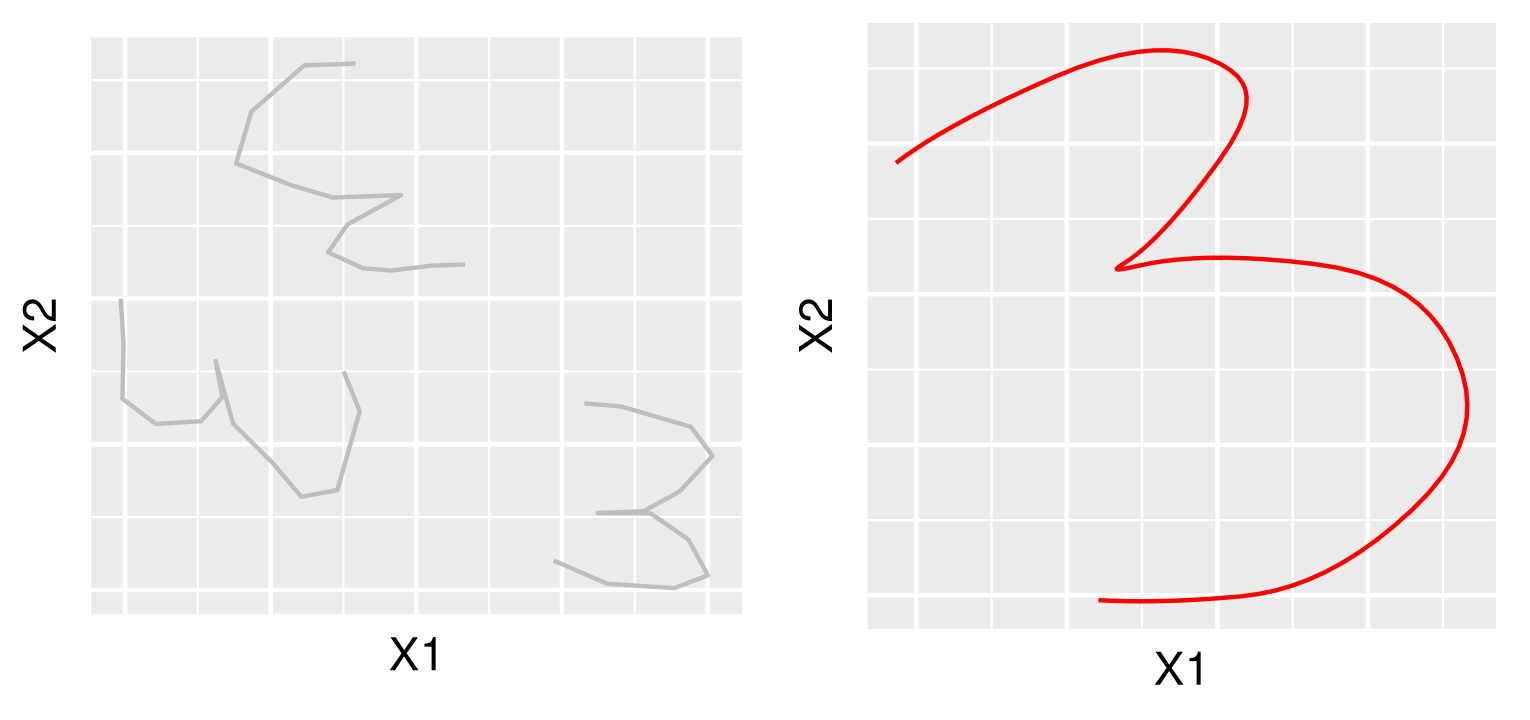
\includegraphics[width=0.7\textwidth]{images/motivation.png}
  \caption{\texttt{digits3.dat} from the \texttt{shapes} package \parencite{shapes} with estimated elastic full Procrustes mean. Data: \textcite{digits3}}
\end{figure}
\vspace{-0.5em}
\textbf{Challenges:}

$\quad$ Sparse and irregular, warping, translation/scaling/rotation
}


% 0-3
%%%%%%%%%%%%%%%%%%%%%%%%%%%%%%%%%%%%%%%%
\frame{
\frametitle{Outline}
\begin{itemize}
  \item[1.] What is an Elastic Full Procrustes Mean?
  %\item[] $\rightarrow$ Sparse and Irregular Planar Curves
  %\item[] $\rightarrow$ Elastic Mean and Warping
  %\item[] $\rightarrow$ Full Procrustes Mean and Procrustes Fits
  \item[2.] Estimation Strategy
  %\item[] $\rightarrow$ Hermitian Covariance Smoothing
  %\item[] $\rightarrow$ Estimation of the Procrustes Mean in a Fixed Basis
  %\item[] $\rightarrow$ Procrustes Fits
  \item[3.] Results (so far), Problems, Outlook
\end{itemize}
}



%%%%%%%%%%%%%%%%%%%%%%%%%%%%%%%%%%%%%%%%
\section{What is an Elastic Full Procrustes Mean?}
%%%%%%%%%%%%%%%%%%%%%%%%%%%%%%%%%%%%%%%%

% 1-1
%%%%%%%%%%%%%%%%%%%%%%%%%%%%%%%%%%%%%%%%
\frame{
\frametitle{Sparse and Irregular Planar Curves}
How can we compare observations $\beta_i = (\beta_{i1}, \beta_{i2}, \dots, \beta_{im_i})$?\\\vspace{0.5em}
$\rightarrow$ Treat $\beta_i$ as \alert{functional} data $\beta_i(t)$: $\,\,\, \beta_i : [0,1] \rightarrow \mathbb{R}^2 $
\begin{columns}
  \begin{column}{0.54\textwidth}
    $\beta_i(t)$ sampled at $t_i = (t_{i1}, \dots, t_{im_i})$:
    $$\beta_{i1} = \beta_i(t_{i1}), \dots, \beta_{im} = \beta_i(t_{im_i})$$
    How to construct $(t_{i1}, \dots, t_{im_i})$?
    \begin{itemize}
      \item simple: arc--length
      \item better: same values of $t$ relate to same "part" of curve
    \end{itemize}
  \end{column}
  \begin{column}{0.46\textwidth}
    \begin{figure}
      \centering
      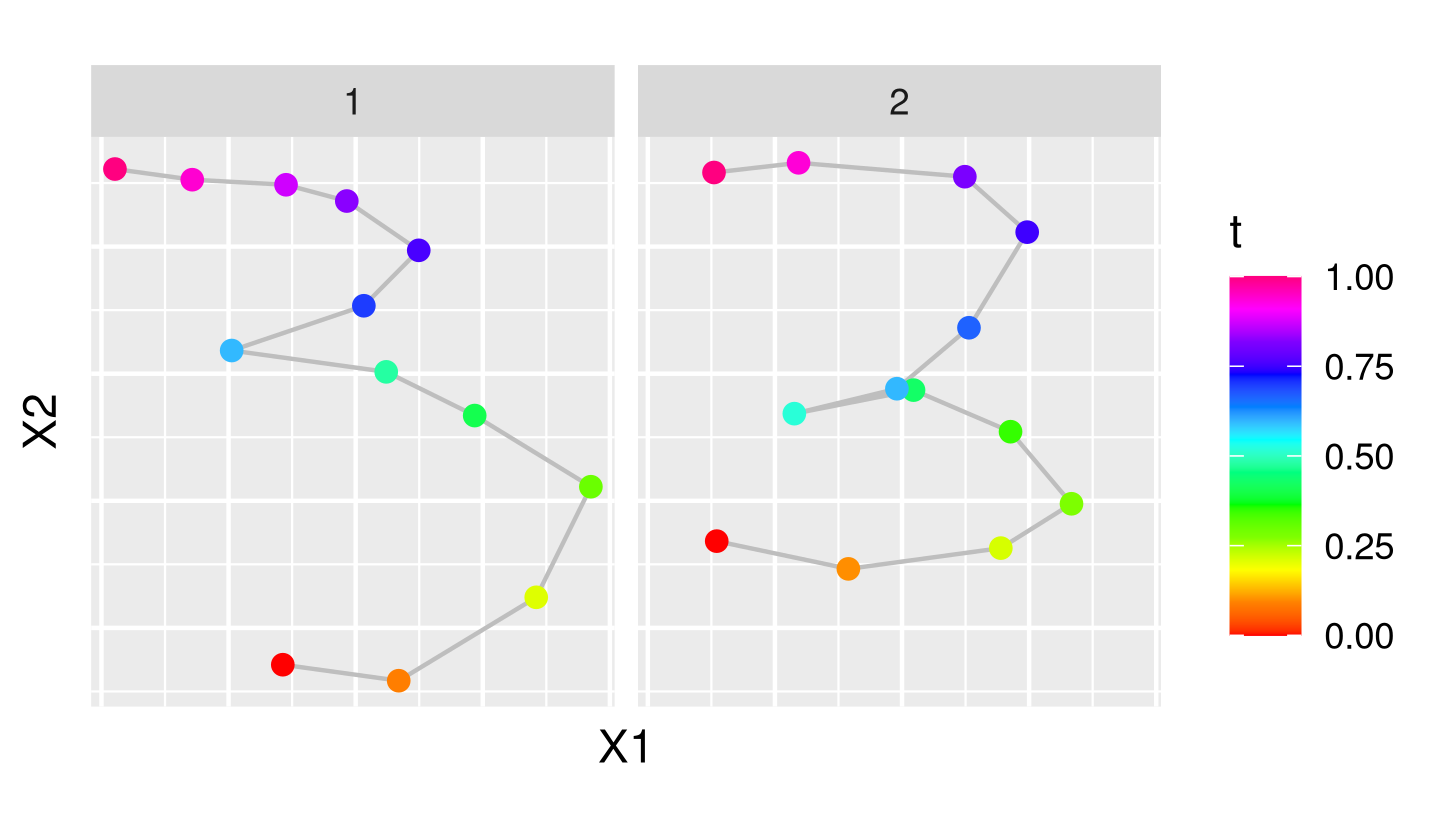
\includegraphics[width=1\textwidth]{images/digits3_arcl.png}
      \vspace{-1.5em}
      \caption{\texttt{digits3.dat} with arc--length parametrisation}
    \end{figure}
  \end{column}
\end{columns}
}



% 1-2
%%%%%%%%%%%%%%%%%%%%%%%%%%%%%%%%%%%%%%%%
\frame{
\frametitle{Elastic Mean and Warping}
\textbf{Problem:} Need to find an optimal re-parametrization (\alert{warping}).

\vspace{0.5em}Well known problem in functional data analysis:
\begin{itemize}
  \item Perform \alert{warping alignment} on SRV curves
\end{itemize}
\begin{block}{Square-Root-Velocity (SRV) Framework \parencite{Srivasta2011}}
$$ q:[0,1] \rightarrow \mathbb{R}^2, \quad 
  q(t) = \frac{\dot{\beta}(t)}{\sqrt{||\dot{\beta}(t)||}} \quad 
  \text{for}\,\,\, ||\dot{\beta}(t)|| \neq 0 $$
\end{block}
\begin{itemize}
  \item Use warping methods for sparse and irregular curves as implemented in \texttt{elasdics} \parencite{elasdics}
  \item Mean under optimal re-parametrization is called \textbf{elastic}
\end{itemize}
}


% 1-3
%%%%%%%%%%%%%%%%%%%%%%%%%%%%%%%%%%%%%%%%
\frame{
\frametitle{Elastic Mean and Warping}
\begin{figure}
  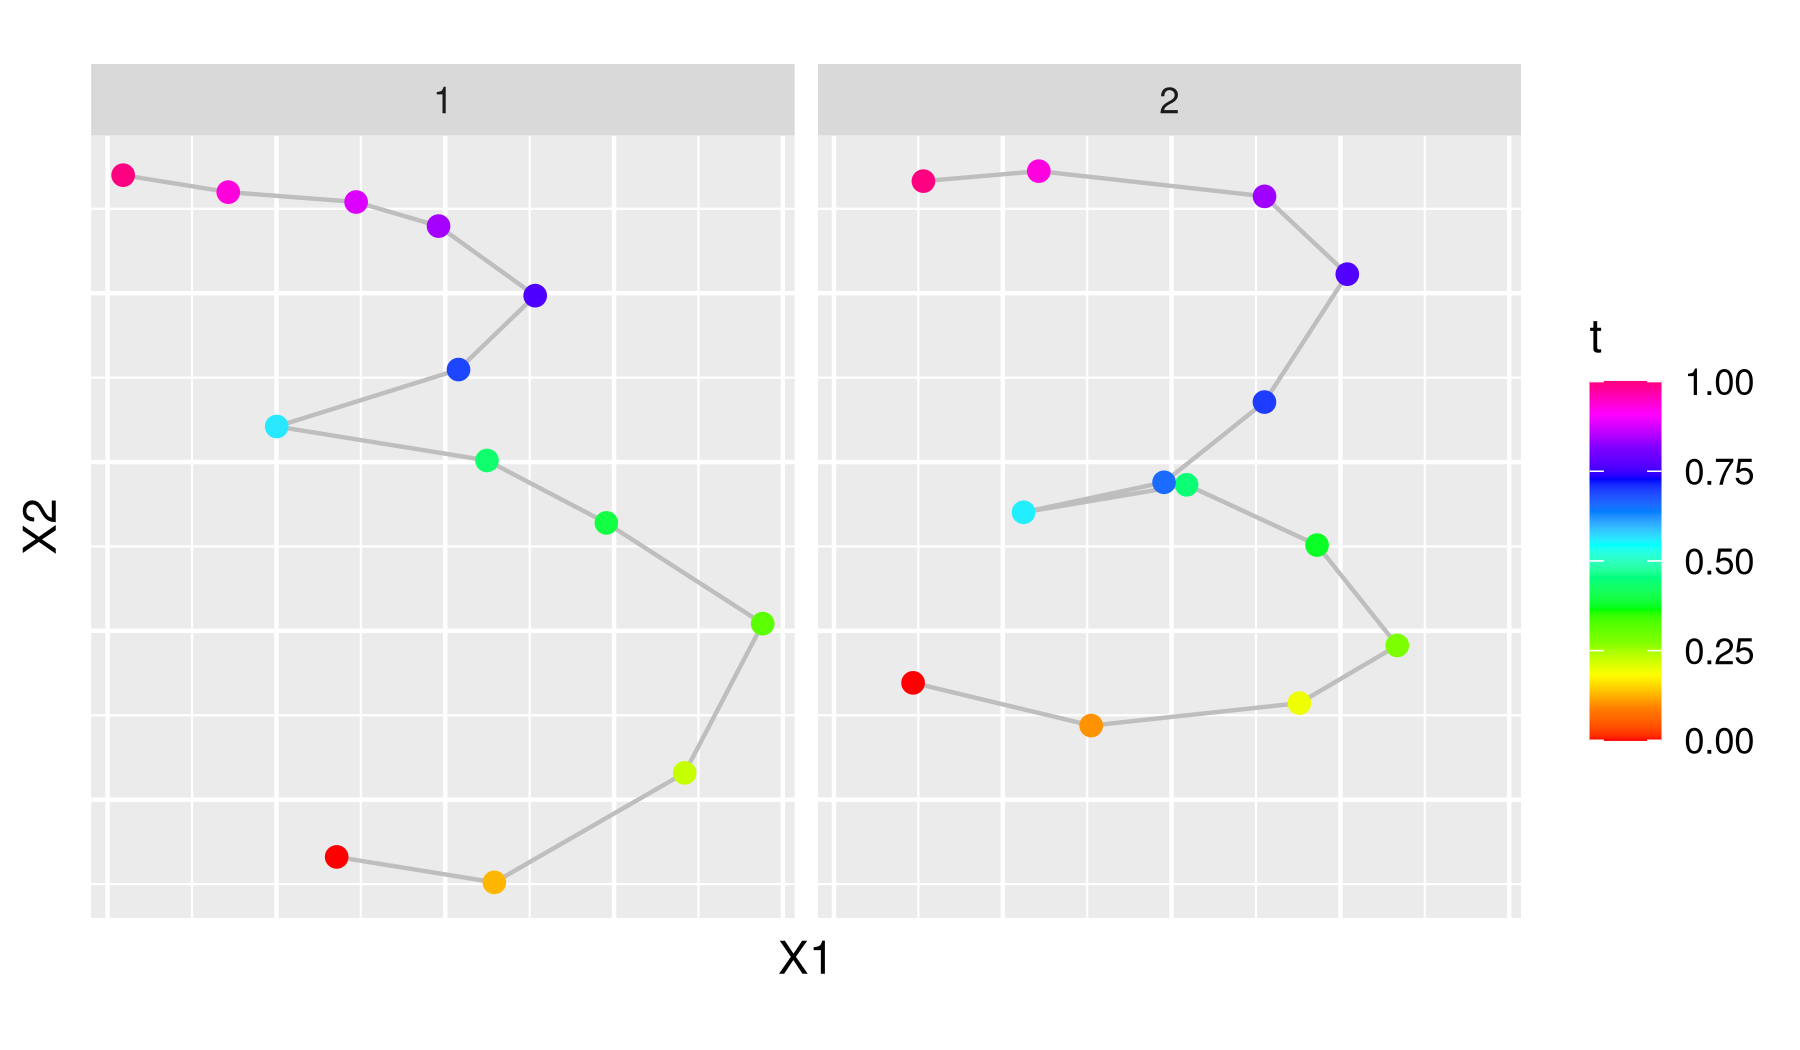
\includegraphics[width=0.7\textwidth]{images/digits3_warp.png}
  \vspace{-0.8em}
  \caption{with \texttt{align\_curves()} from package \texttt{elasdics} \parencite{elasdics}}
\end{figure}
\vspace{-0.3em}
\alert{Problem}: Methods are not invariant under rotation/scaling!
}



\frame{
\frametitle{Full Procrustes Mean and Procrustes Fits}
\vspace{-0.3em}
\textbf{Basic idea:}
\begin{itemize}
  \item[1.] Calculate mean that is invariant under rotation, scaling
  \item[2.] Align rotation and scaling 
  \item[3.] Align parametrisation 
  \item[$\rightarrow$] use estimated mean as reference for alignment
\end{itemize}
%\vspace{-0.5em}
%\begin{figure}
%\hspace{-3em}
%\begin{subfigure}{.33\textwidth}
%  \centering
%  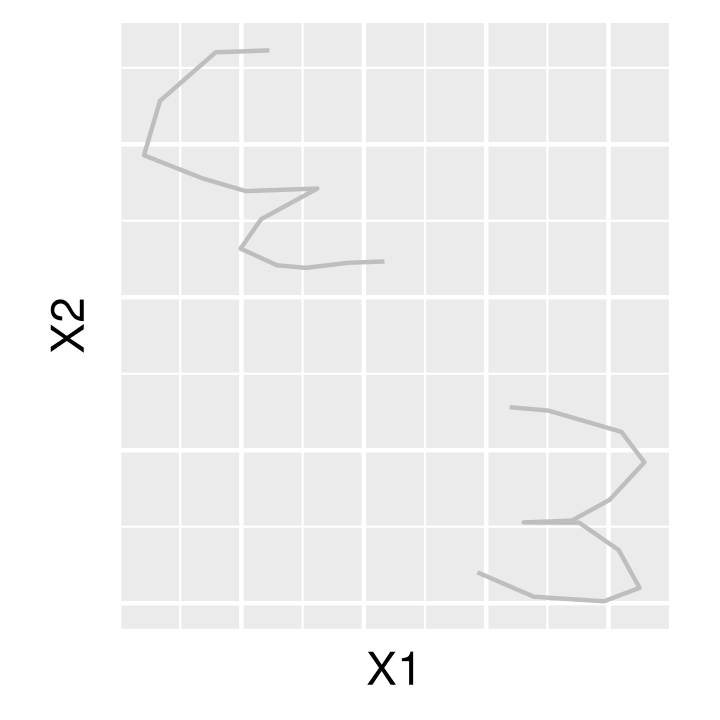
\includegraphics[width=.8\linewidth]{images/basic1.png}
%\end{subfigure}$\overset{1.}{\rightarrow}$%
%\begin{subfigure}{.33\textwidth}
%  \centering
%  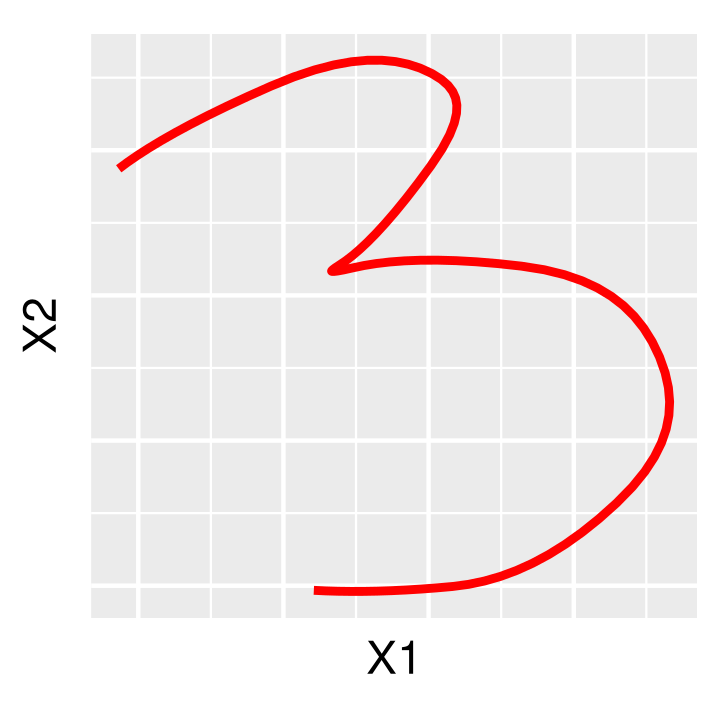
\includegraphics[width=.8\linewidth]{images/basic2.png}
%\end{subfigure}$\overset{2}{\rightarrow}$%
%\begin{subfigure}{.33\textwidth}
%  \centering
%  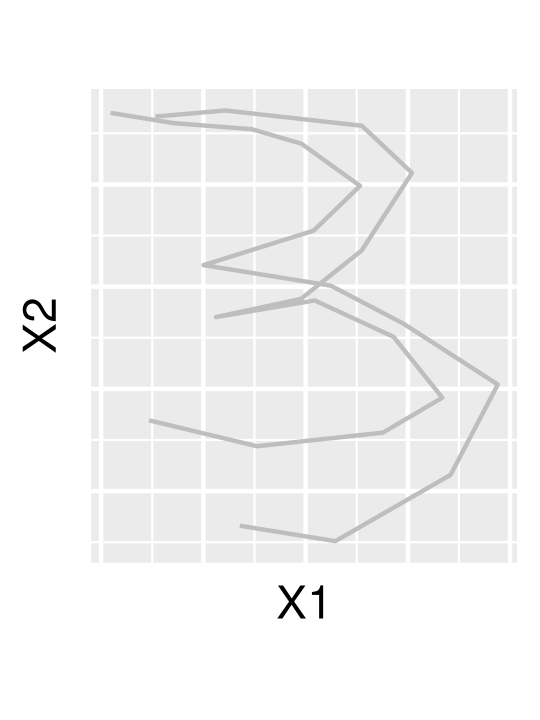
\includegraphics[width=.8\linewidth]{images/basic3.png}
%\end{subfigure}$\overset{3.}{\rightarrow}$
%\end{figure}
%\vspace{-1.2em}
\vspace{1em}
1+2 are known problems in \textbf{statistical shape analysis} (see e.g. \textcite{DrydenMardia2016})
$\,\rightarrow$ \alert{Procrustes mean} and \alert{Procrustes fits}

\vspace{1.2em}
\textbf{Note:} More efficient to perform steps directly on the SRV curves!

}


% 1-4
%%%%%%%%%%%%%%%%%%%%%%%%%%%%%%%%%%%%%%%%
\frame{
\frametitle{Full Procrustes Mean and Procrustes Fits}
\textbf{Now:} Need to derive the Procrustes mean for functional data

\vspace{0.8em}We can show using \alert{complex} notation 
$$\,\, q_i : [0,1] \rightarrow \mathbb{C}, \quad q_i(t) = x_i(t) + i \, y_i(t)$$
that the population level \alert{full Procrustes mean} for normalized curves $\tilde{q}$ is given by:
$$\mu_q = \argmax_{z:[0,1] \rightarrow \mathbb{C},\,||z||=1} \int_0^1 \int_0^1 \overline{z}(s)\, \mathbb{E}\left[\tilde{q}(s) \overline{\tilde{q}}(t) \right] z(t) ds dt$$
\begin{itemize}
  \item[$\rightarrow$] $\mathbb{E}\left[\tilde{q}(s) \overline{\tilde{q}}(t) \right]$ is the \alert{complex covariance function} $C(s,t)$
\end{itemize}
}


% 1-9
%%%%%%%%%%%%%%%%%%%%%%%%%%%%%%%%%%%%%%%%
\frame{
\frametitle{Full Procrustes Mean and Procrustes Fits}
\textbf{Population level full Procrustes mean:}
$$\mu_q = \argmax_{z:[0,1] \rightarrow \mathbb{C},\, ||z|| = 1} \int_0^1 \int_0^1 \overline{z}(s) C(s,t) z(t) ds dt$$
\vspace{-0.5em}
\begin{itemize}
  \item[$\rightarrow$] \alert{Functional PCA} problem (see \textcite{RamsaySilverman2005})
  \item[$\rightarrow$] Solution is the leading complex eigenfunction of $C(s,t)$
  \item[$\rightarrow$] We only need to find a good estimate $\alert{\hat{C}(s,t)}$ to get $\hat{\mu}_q$!
\end{itemize}
\vspace{1em}
\textbf{Procrustes fits}:
$$\hat{q}^P_i = \langle \tilde{q}_i, \hat{\mu}_q \rangle \tilde{q}_i$$
with $\langle f, g \rangle = \int_0^1 \overline{f(t)} g(t) dt$
}



\section{Estimation Strategy}

% 2-1
%%%%%%%%%%%%%%%%%%%%%%%%%%%%%%%%%%%%%%%%
\frame{
\frametitle{Hermitian Covariance Smoothing}
Treat estimation of $C(s,t) = \mathbb{E}[ \tilde{q}(s) \overline{\tilde{q}}(t)]$ as a regression problem:
\vspace{0.5em}
\begin{itemize}
  \item we can build response $y_{ijk} = \tilde{q}_i(t_{ij}) \overline{\tilde{q}}_i(t_{ik})$
  \item treat parametrisation $t_{ij}, t_{ik}$ as \enquote{covariates} $s$ and $t$
  \item non-parametric regression:  $\mathbb{E}[y] = f(s,t)$
  \item use $\hat{C}(s,t) = \hat{f}(s,t)$ for functional PCA
\end{itemize}

\vspace{1em}
\alert{Note}: Using symmetry properties of $C(s,t)$ is important for efficient estimation (see \textcite{Cederbaum2018}).

\vspace{0.5em}
$\rightarrow$ use every combination $(t_{ij}, t_{ik})$ only once
}


% 2-2
%%%%%%%%%%%%%%%%%%%%%%%%%%%%%%%%%%%%%%%%
\frame{
\frametitle{Hermitian Covariance Smoothing}

\textbf{Here:} Complex covariance function is \alert{hermitian} $C(s,t) = \overline{C}(t,s)$
$$\mathbb{E}[Re(y)] = f_{symm}(s,t)$$
$$\mathbb{E}[Im(y)] = f_{skew}(s,t)$$
\vspace{-1.2em}
\begin{itemize}
  \item model real and imaginary parts seperately using e.g.\ \texttt{mgcv} \parencite{Wood2017}
  \item with \alert{symmetric} and \alert{skew-symmetric} tensor product P-splines from \texttt{sparseFLMM} \parencite{sparseFLMM}
\end{itemize}
\vspace{0.5em}
\textbf{We get:}
$$\hat{C}(s,t) = b(s)^T \hat{\Xi} b(t), \quad \text{with} \quad \hat{\Xi} = \hat{\Xi}_{symm} + i \, \hat{\Xi}_{skew}$$
}


% 2-2
%%%%%%%%%%%%%%%%%%%%%%%%%%%%%%%%%%%%%%%%
\frame{
\frametitle{Hermitian Covariance Smoothing}
\begin{figure}
  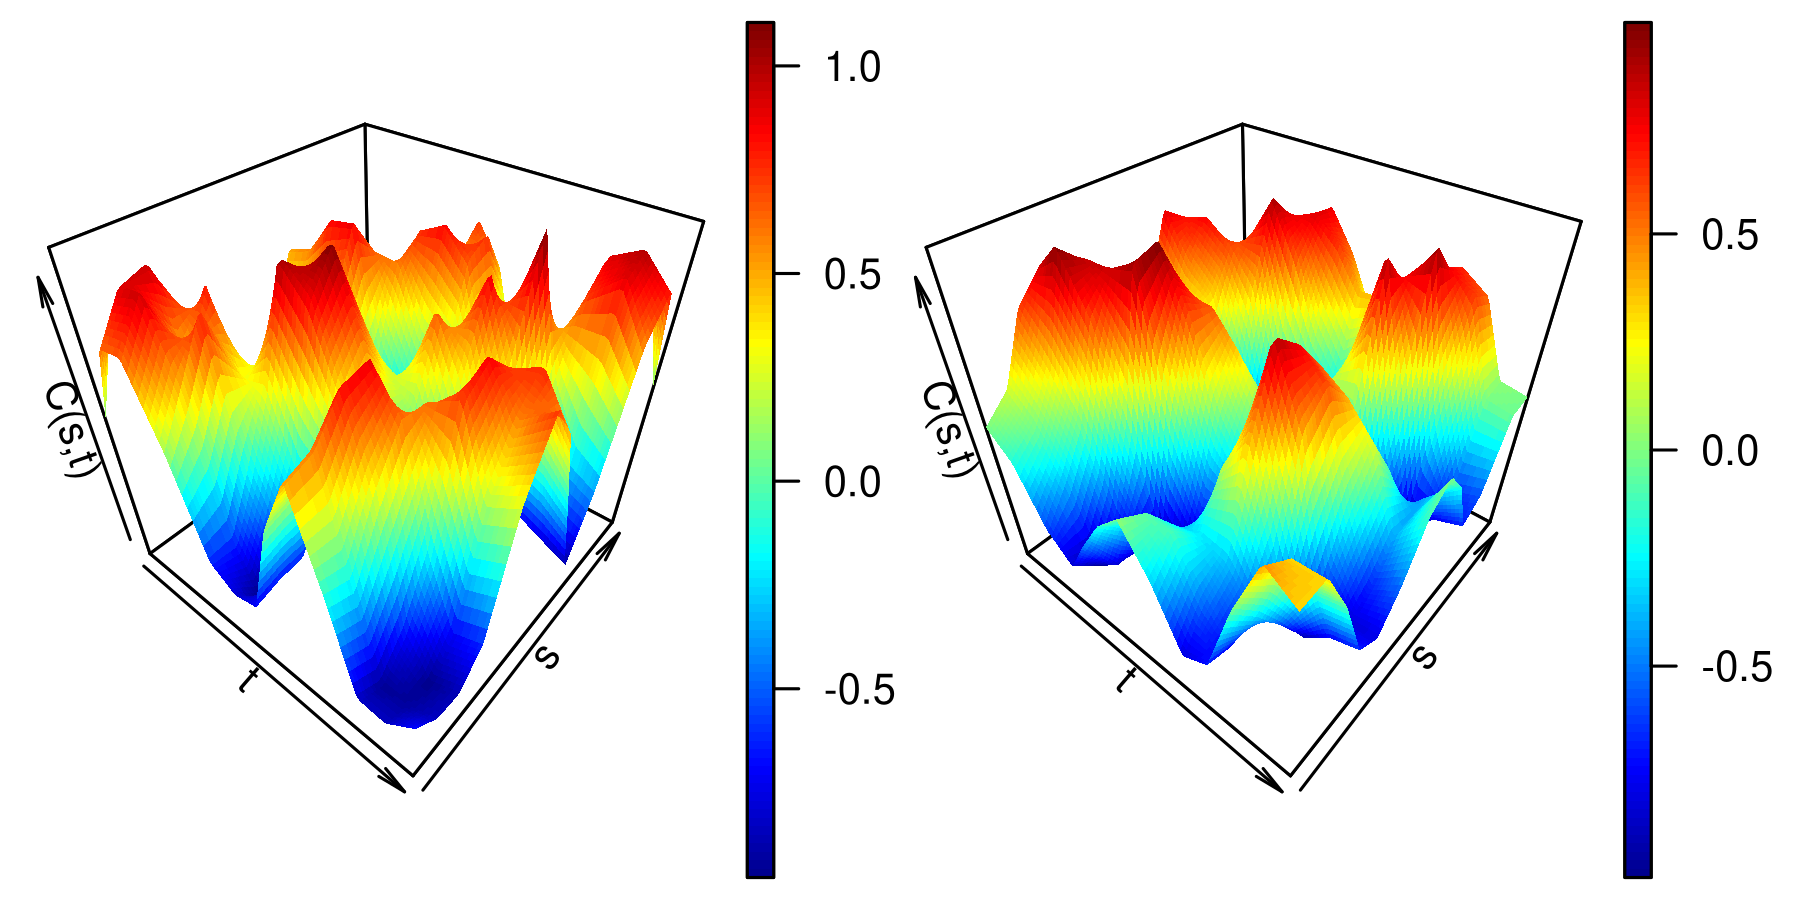
\includegraphics[width=0.75\textwidth]{images/cov_surface_smooth.png}
  \caption{Estimated real (left) and imaginary (right) parts of $C(s,t)$}
\end{figure}
}

% 2-3
%%%%%%%%%%%%%%%%%%%%%%%%%%%%%%%%%%%%%%%%
\frame{
\frametitle{Empirical Procrustes Mean in a Fixed Basis}
\textbf{Idea:} Estimate covariance function and mean in the same basis.

\vspace{1em}
Then the optimization problem reduces to:
$$\hat\theta_\mu = \argmax_{\theta : \theta^H G \theta = 1} \theta^H G \hat{\Xi} G \theta \quad \text{with} \quad G_{kl} = \langle b_k, b_l \rangle $$
Eigenvalue problem treating $\theta = \theta_{Re} + i \, \theta_{Im}$ seperately:
$$ \begin{pmatrix}
  \hat{\Xi}_{symm} & - \hat{\Xi}_{skew}\\
  \hat{\Xi}_{skew} & \hat{\Xi}_{symm}
\end{pmatrix}
\begin{pmatrix}
  G & 0 \\
  0 & G 
\end{pmatrix}
\begin{pmatrix}
  \theta_{Re} \\
  \theta_{Im}
\end{pmatrix}
= \lambda
\begin{pmatrix}
  \theta_{Re} \\
  \theta_{Im}
\end{pmatrix}
$$
$\Rightarrow$ Solution is the leading normalized eigenvector of $\underline{\hat{\Xi}} \underline{G}$\\
}


% 2-4
%%%%%%%%%%%%%%%%%%%%%%%%%%%%%%%%%%%%%%%%
\frame{
\frametitle{Procrustes Fits}
After obtaining $\hat{\mu}_q$ we can estimate the Procrustes fits:
$$\hat{q}^P_i = \alert{\langle \tilde{q}_i, \hat{\mu}_q \rangle} \tilde{q}_i$$
\vspace{-1.2em}
\begin{itemize}
  \item at the moment: integration with linear interpolation of $\tilde{q}_i$'s
  \item alternative: smoothing in mean basis with $\langle \hat{\tilde{q}}_i, \hat\mu_q \rangle = \hat{\theta}^H_i G \hat{\theta}_\mu$
\end{itemize}
\begin{figure}
  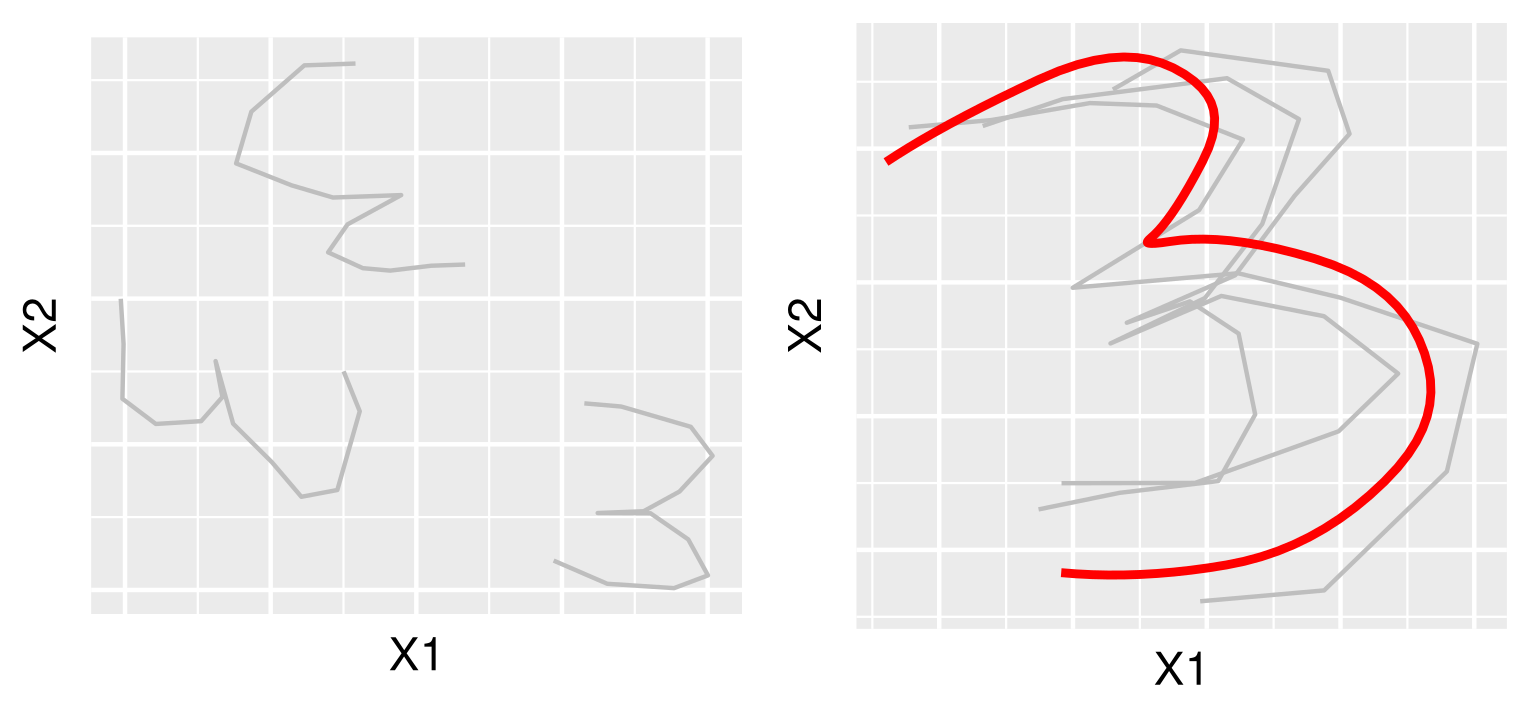
\includegraphics[width=0.75\textwidth]{images/pfit_mean_digits3.png}
  \vspace{-1em}
  \caption{Procrustes fits and mean (on full dataset) before warping.}
\end{figure}
}



\section{Results, Problems, Outlook}
% 3-1
%%%%%%%%%%%%%%%%%%%%%%%%%%%%%%%%%%%%%%%%
\frame{
\frametitle{Results}
\begin{figure}
  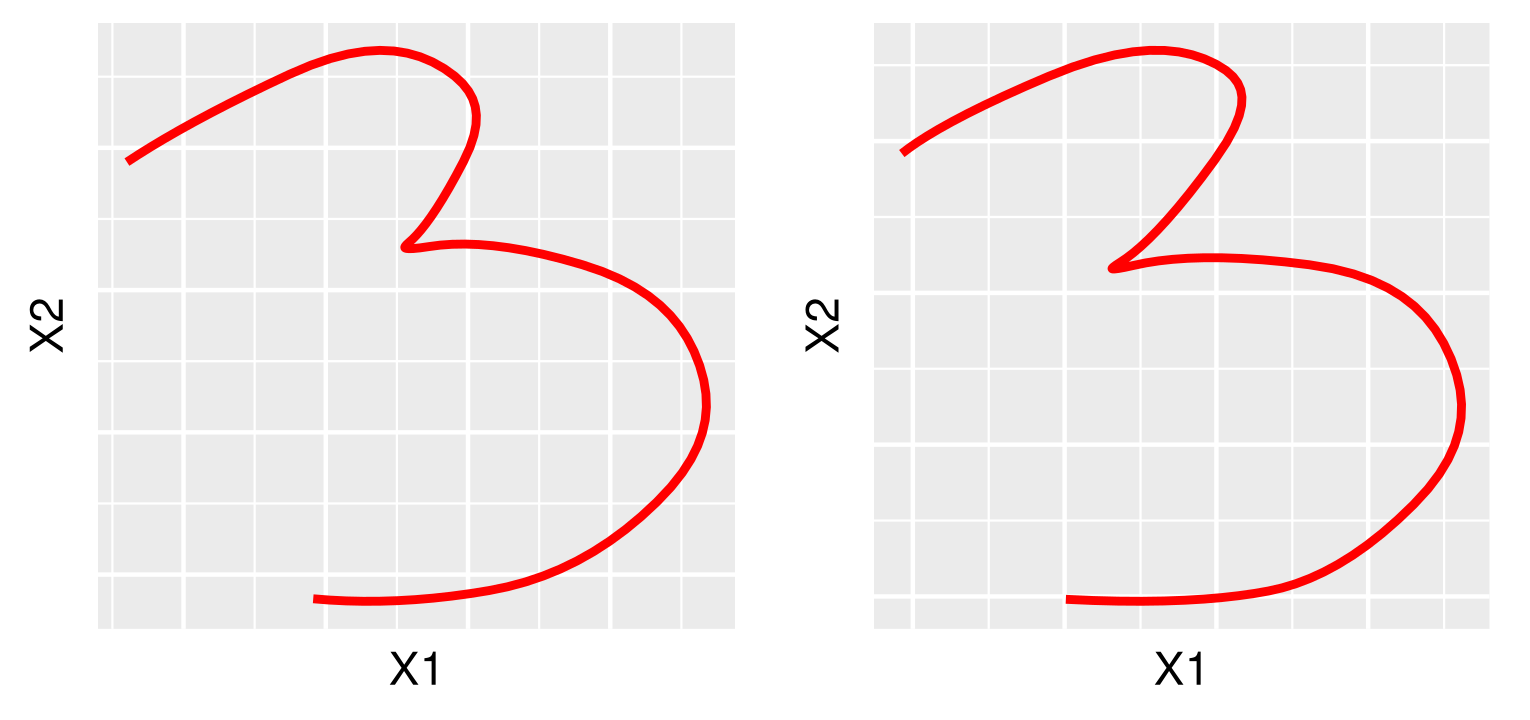
\includegraphics[width=0.85\textwidth]{images/results_digits3_warp.png}
  \caption{Full Procrustes mean (left) and elastic full Procrustes mean (right) on \texttt{digits3.dat}.}
\end{figure}
}


% 3-2
%%%%%%%%%%%%%%%%%%%%%%%%%%%%%%%%%%%%%%%%
\frame{
\frametitle{Results / Problems}
\begin{figure}
  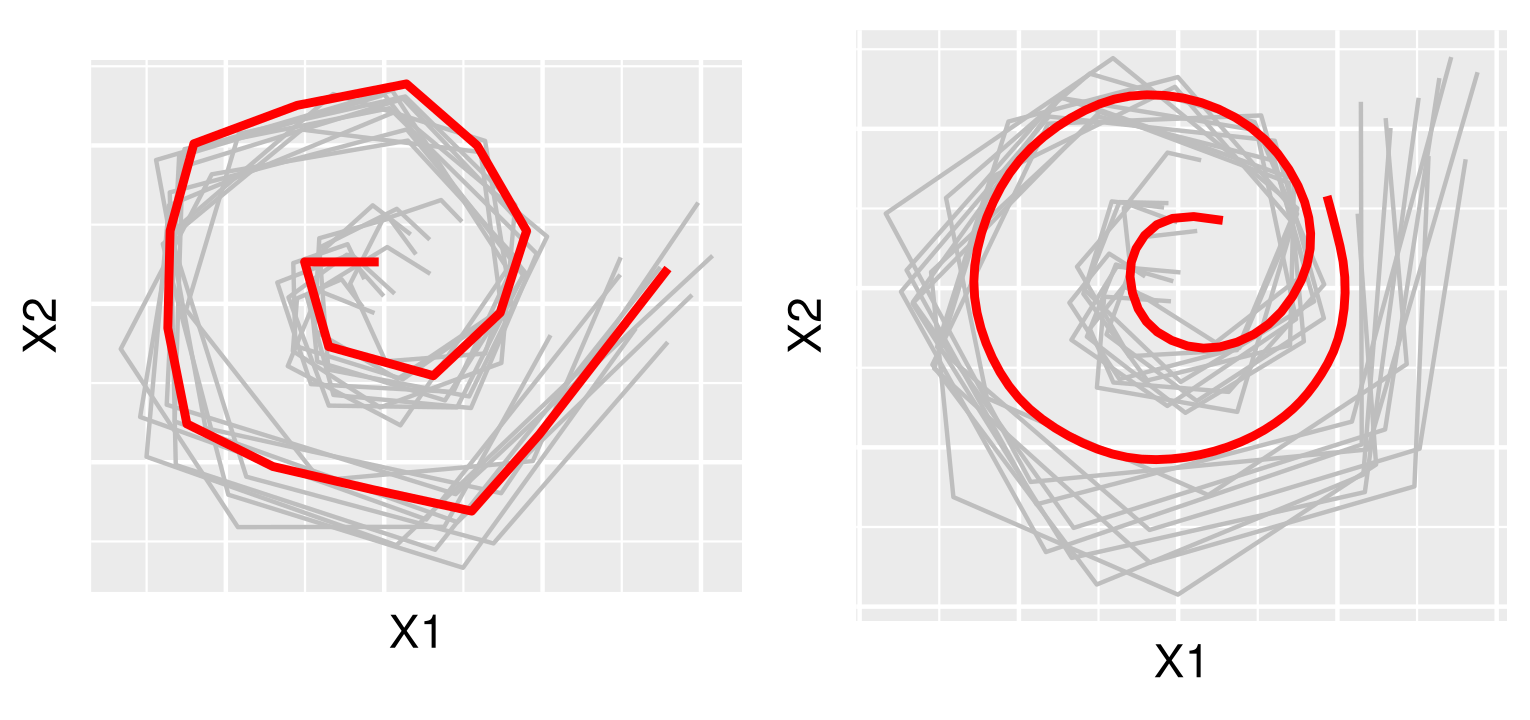
\includegraphics[width=0.8\textwidth]{images/results_spirals.png}
  \vspace{-1em}
  \caption{Polygon (left) and smooth (right) elastic full Procrustes mean with procrustes fits.}
\end{figure}
\vspace{-0.5em}
\begin{itemize}
  \item[$\rightarrow$] Parameters: \textbf{knots}, \textbf{spline degree}, \textbf{penalty} 
  \item[$\rightarrow$] Consistent results for piecewise constant splines (at SRV level) and zero order penalty (in the cov.\ estimation).
\end{itemize}
}


% 3-4
%%%%%%%%%%%%%%%%%%%%%%%%%%%%%%%%%%%%%%%%
\frame{
\frametitle{Outlook}
\textbf{Next steps:}
\begin{itemize}
  \item Real world data application (open curves)
  \item Better normalization / estimation of procrustes fits
\end{itemize}
\vspace{1em}
\textbf{Nice to have (maybe later):}
\begin{itemize}
  \item Mean for closed curves
  \item \textbf{Code}: bugs, testcases, faster
\end{itemize}
}

% Appendix
%%%%%%%%%%%%%%%%%%%%%%%%%%%%%%%%%%%%%%%
\section{Appendix}
\nocite{*}
\frame[allowframebreaks]{
\printbibliography
}

% 2-5
%%%%%%%%%%%%
\renewcommand{\algorithmicrequire}{\textbf{Input:}}
\renewcommand{\algorithmicensure}{\textbf{Output:}}

\frame{
\frametitle{Putting it all together}
\vspace{-0.8em}
\begin{algorithm}[H]
\caption{Elastic Full Procrustes Mean}
\begin{algorithmic}[1]
\Require{Data curves $\beta_1, \dots, \beta_N$}
\Ensure{Procrustes mean $\hat{\mu}$ and Procrustes fits $\hat{\beta}_1^P, \dots, \hat{\beta}_N^P$}
  \Statex
  \State {initialize arc--length parametrisation $t_i$ for all $\beta_i$}
  \State {calculate normalized SRV curves $\tilde{q}_i = \frac{q_i}{||q_i||}$}
  \While{convergence not reached}
    \State {estimate $C(s,t)$ using $t_i$}
    \State {calculate $\hat{\mu}_q$ as the leading eigenfunction of $\hat{C}(s,t)$}
    \State {estimate Procrustes fits $\tilde{q}_i^P$}
    \State {update $t_i \leftarrow t_i^{optim}$ using warping alignment on $\hat{\tilde{q}}_i^P$}
  \EndWhile
  \State \Return {integrated Procrustes mean and fits}
\end{algorithmic}
\end{algorithm}
}


% 3-3
%%%%%%%%%%%%%%%%%%%%%%%%%%%%%%%%%%%%%%%%
\frame{
\frametitle{Problems}
\textbf{Normalization:} $\tilde{q}_i = \frac{q_i}{||q_i||}$ is itself an estimate ($||q_i|| = \sqrt{\alert{\langle q_i, q_i \rangle}}$)
\vspace{0.5em}
\begin{itemize}
  \item[$\rightarrow$] can either restrict $\beta_i$'s to unit--length or normalize $q_i$ directly
\end{itemize}
\vspace{-0.3em}
\begin{figure}
  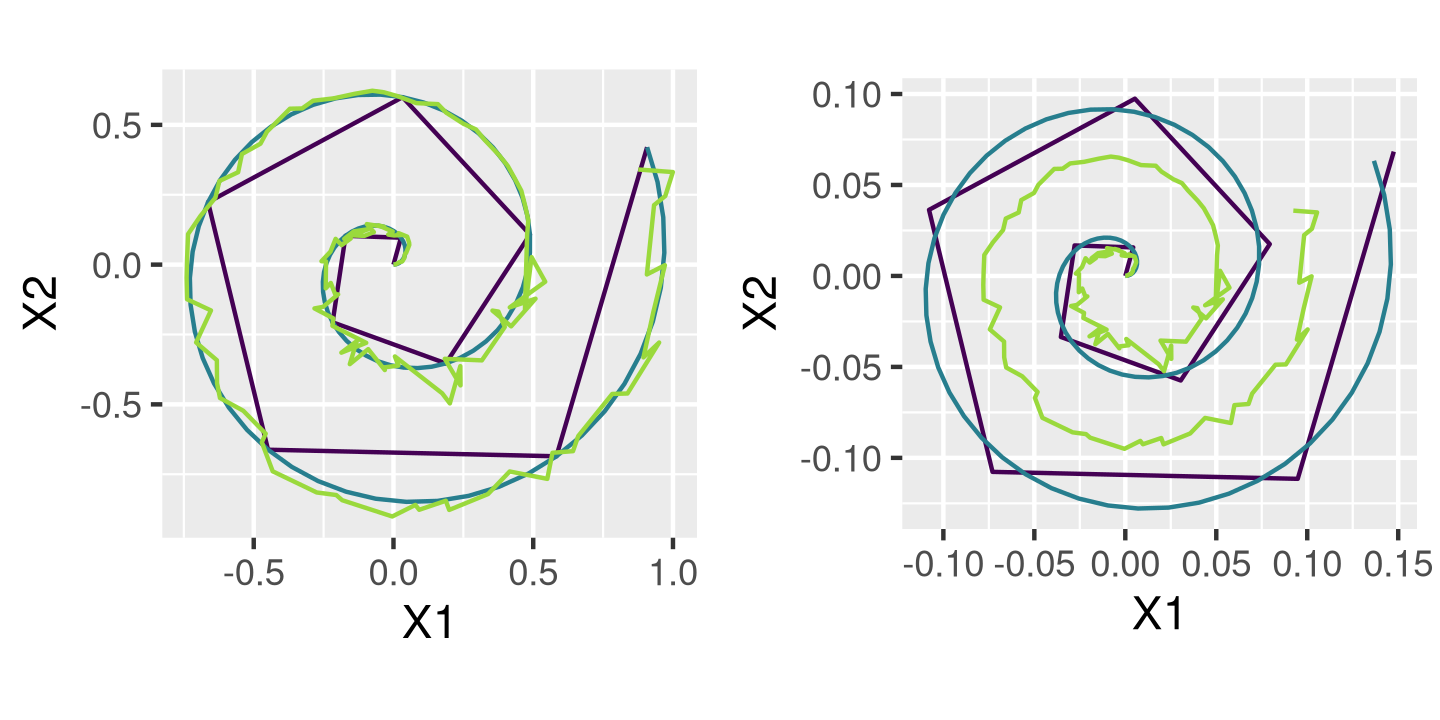
\includegraphics[width=0.7\textwidth]{images/normalization.png}
  \vspace{-1.3em}
  \caption{Spirals (left) and unit--length spirals (right).}
\end{figure}
\vspace{-0.5em}
\begin{itemize}
  \item[$\rightarrow$] likely need smoothing (in the mean basis?) for this
  \item[$\rightarrow$] only ok, as long as all curves have same "amount" of sparsity 
\end{itemize}
}




\frame{
\frametitle{Derivation: Empirical Full Procrustes Mean}
\begin{block}{Full Procrustes Distance and Mean}
  $$d_F(q_1, q_2) = \inf_{\Gamma, b} ||q_1 - b \Gamma q_2||$$
  \vspace{-1.5em}
  $$\mu_q : [0,1] \rightarrow \mathbb{R}^2, \quad \hat{\mu}_q = \argmin_{z : [0,1] \rightarrow \mathbb{R}^2} \sum_{i=1}^N d_F(z, q_i)^2$$
\end{block}
One can show that \parencite[see Ch.\ 8]{DrydenMardia2016}:
$$\hat{\mu}_q = \argmin_{z : [0,1] \rightarrow \mathbb{C}} \sum_{i=1}^N
    \underbrace{1 - \frac{\langle z, q_i \rangle \langle q_i, z \rangle}{\langle z, z \rangle \langle q_i, q_i \rangle}}_{= d_F(z, q_i)^2}$$
}


\frame{
\frametitle{Derivation: Empirical Full Procrustes Mean}
\alert{Note}: $\langle q_1, q_2 \rangle = \int_0^1 \overline{q}_1(t) q_2(t) dt, \quad \text{and} \quad ||q_i|| = \sqrt{\langle q_i, q_i \rangle}$
\begin{align*}
 \hat{\mu}_q  &= \argmax_{z : ||z|| = 1} \sum_{i=1}^N \langle z, \tilde{q}_i \rangle \langle \tilde{q}_i, z \rangle, \quad \text{\alert{with}} \quad \tilde{q}_i = \frac{q_i}{||q_i||}\\ 
  &= \argmax_{z:||z|| = 1} \sum_{i=1}^N \int_0^1 \overline{z}(s) \tilde{q}_i(s) ds \int_0^1 \overline{\tilde{q}}_i(t) z(t) dt \\
  &= \argmax_{z:||z||=1} \int_0^1 \int_0^1 \overline{z}(s) \left( \alert{\sum_{i=1}^N \tilde{q}_i(s) \overline{\tilde{q}}_i(t)} \right) z(t) ds dt
\end{align*}
\begin{itemize}
  \item[$\rightarrow$] sample analouge to $C(s,t) = \mathbb{E}[ \tilde{q}(s) \overline{\tilde{q}}(t)]$ 
\end{itemize}
}


\frame{
\frametitle{Derivation: Mean in a Fixed Basis}
$$\mu_q = \argmax_{z:[0,1] \rightarrow \mathbb{C},\, ||z|| = 1} \int_0^1 \int_0^1 \overline{z}(s) C(s,t) z(t) ds dt$$
\vspace{0.5em}
with $z(t) = b(t)^T\theta$ and $\hat{C}(s,t) = b(s)^T \hat{\Xi} b(t)$. Then
\begin{align*}
  \hat{\theta}_\mu =& \argmax_{\theta : ||b^T\theta||=1} \int_0^1 \int_0^1 \overline{\left(b(s)^T\theta\right)} b(s)^T \hat{\Xi} b(t) b(t)^T \theta \, ds dt \\
  =& \argmax_{\theta: ||b^T\theta||=1} \theta^H \left(\int_0^1 b(s) b(s)^T ds\right) \hat{\Xi} \left( \int_0^1 b(t) b(t)^T dt \right) \theta\\
  = & \argmax_{\theta: ||b^T\theta||=1} \theta^H G \hat{\Xi} G \theta
\end{align*}
\alert{Note:} $||b^T\theta|| = \sqrt{\theta^H G \theta}$
}


\end{document}
